% !TEX TS-program = pdfLaTeX+MakeIndex+BibTeX
% !TEX encoding = UTF-8 Unicode

\PassOptionsToPackage{unicode}{hyperref}
\PassOptionsToPackage{naturalnames}{hyperref}

\documentclass[tg]{mdtufsm}

\usepackage[T1]{fontenc}
\usepackage{fix-cm}
\usepackage{url}
\usepackage{times, color}
\usepackage[utf8]{inputenc}
\usepackage{graphicx}
\usepackage{amsmath,latexsym,amssymb}
%\usepackage[hidelinks]{hyperref}
\usepackage[hidelinks,
            bookmarksopen=true,linktoc=none,colorlinks=true,
            linkcolor=black,citecolor=black,filecolor=magenta,urlcolor=blue,
            pdftitle={Automatização do Gerenciamento e Implantação de Instâncias AWS EC2 para Ensino de Computação Distribuída},
            pdfauthor={Cezar Augusto Contini Bernardi},
            pdfsubject={Trabalho de Graduação},
            pdfkeywords={Cloud computing, orquestração, computação distribuída, ensino, UFSM}
            ]{hyperref}
            
%\usepackage[brazilian]{babel}

%\usepackage{fontspec}
%\setmainfont{Linux Libertine G}

%%% PAGE DIMENSIONS
\usepackage[inner=30mm,outer=20mm,top=30mm,bottom=20mm]{geometry} 
\usepackage{epstopdf}
\usepackage{graphicx}
\usepackage{pdfpages}
% \geometry{margin=2in} % for example, change the margins to 2 inches all round
% \geometry{landscape} % set up the page for landscape

% \usepackage[parfill]{parskip} % Activate to begin paragraphs with an empty line rather than an indent

%%% PACKAGES
%\usepackage{amsfonts}
\usepackage{color}
%\usepackage{booktabs} % for much better looking tables
%\usepackage{array} % for better arrays (eg matrices) in maths
%\usepackage{paralist} % very flexible & customisable lists (eg. enumerate/itemize, etc.)
\usepackage{verbatim} % adds environment for commenting out blocks of text & for better verbatim
\usepackage{listings}
\usepackage{parcolumns}
\usepackage{siunitx}
%\usepackage{verbatim} % adds environment for commenting out blocks of text & for better verbatim
\usepackage{subcaption}
\captionsetup{compatibility=false}
%\usepackage{microtype}
%\usepackage[numbers]{natbib}
%\usepackage{subfig} % make it possible to include more than one captioned figure/table in a single float
% These packages are all incorporated in the memoir class to one degree or another...

\definecolor{codegreen}{rgb}{0,0.6,0}
\definecolor{codegray}{rgb}{0.5,0.5,0.5}
\definecolor{codepurple}{rgb}{0.58,0,0.82}
\definecolor{backcolour}{rgb}{0.95,0.95,0.92}
\lstdefinestyle{mystyle}{
	backgroundcolor=\color{backcolour},   commentstyle=\color{codegreen},
	keywordstyle=\color{magenta},
	numberstyle=\tiny\color{codegray},
	stringstyle=\color{codepurple},
	basicstyle=\footnotesize,
	breakatwhitespace=false,         
	breaklines=true,                 
	captionpos=b,                    
	keepspaces=true,                 
	numbers=left,                    
	numbersep=5pt,                  
	showspaces=false,                
	showstringspaces=false,
	showtabs=false,                  
	tabsize=2,
	literate=
	{á}{{\'a}}1 {é}{{\'e}}1 {í}{{\'i}}1 {ó}{{\'o}}1 {ú}{{\'u}}1
	{Á}{{\'A}}1 {É}{{\'E}}1 {Í}{{\'I}}1 {Ó}{{\'O}}1 {Ú}{{\'U}}1
	{à}{{\`a}}1 {è}{{\`e}}1 {ì}{{\`i}}1 {ò}{{\`o}}1 {ù}{{\`u}}1
	{À}{{\`A}}1 {È}{{\'E}}1 {Ì}{{\`I}}1 {Ò}{{\`O}}1 {Ù}{{\`U}}1
	{ä}{{\"a}}1 {ë}{{\"e}}1 {ï}{{\"i}}1 {ö}{{\"o}}1 {ü}{{\"u}}1
	{Ä}{{\"A}}1 {Ë}{{\"E}}1 {Ï}{{\"I}}1 {Ö}{{\"O}}1 {Ü}{{\"U}}1
	{â}{{\^a}}1 {ê}{{\^e}}1 {î}{{\^i}}1 {ô}{{\^o}}1 {û}{{\^u}}1
	{Â}{{\^A}}1 {Ê}{{\^E}}1 {Î}{{\^I}}1 {Ô}{{\^O}}1 {Û}{{\^U}}1
	{ã}{{\~a}}1 {Ã}{{\~A}}1
	{ç}{{\c c}}1 {Ç}{{\c C}}1
}

\lstset{style=mystyle}
\iffalse

\lstdefinelanguage{python}{
	keywords={typeof, null, catch, switch, in, int, str, float, self},
	%keywordstyle=\color{ForestGreen}\bfseries,
	ndkeywords={boolean, throw, import},
	ndkeywords={return, class, if ,elif, endif, while, do, else, True, False , catch, def},
	%ndkeywordstyle=\color{BrickRed}\bfseries,
	i%dentifierstyle=\color{black},
	sensitive=false,
	comment=[l]{\#},
	morecomment=[s]{/*}{*/},
	%commentstyle=\color{purple}\ttfamily,
	%stringstyle=\color{red}\ttfamily,
}
\lstset{
	basicstyle=\scriptsize\ttfamily,
	tabsize=2,
	frame=single,
	breaklines=true,
	breakatwhitespace=true,
	xleftmargin=0cm,
	xrightmargin=0cm,
	literate=
		{á}{{\'a}}1 {é}{{\'e}}1 {í}{{\'i}}1 {ó}{{\'o}}1 {ú}{{\'u}}1
		{Á}{{\'A}}1 {É}{{\'E}}1 {Í}{{\'I}}1 {Ó}{{\'O}}1 {Ú}{{\'U}}1
		{à}{{\`a}}1 {è}{{\`e}}1 {ì}{{\`i}}1 {ò}{{\`o}}1 {ù}{{\`u}}1
		{À}{{\`A}}1 {È}{{\'E}}1 {Ì}{{\`I}}1 {Ò}{{\`O}}1 {Ù}{{\`U}}1
		{ä}{{\"a}}1 {ë}{{\"e}}1 {ï}{{\"i}}1 {ö}{{\"o}}1 {ü}{{\"u}}1
		{Ä}{{\"A}}1 {Ë}{{\"E}}1 {Ï}{{\"I}}1 {Ö}{{\"O}}1 {Ü}{{\"U}}1
		{â}{{\^a}}1 {ê}{{\^e}}1 {î}{{\^i}}1 {ô}{{\^o}}1 {û}{{\^u}}1
		{Â}{{\^A}}1 {Ê}{{\^E}}1 {Î}{{\^I}}1 {Ô}{{\^O}}1 {Û}{{\^U}}1
		{ã}{{\~a}}1 {Ã}{{\~A}}1
		{ç}{{\c c}}1 {Ç}{{\c C}}1
}
\fi

% For Computer Modern:
%\def\Cpp{{C\nolinebreak[4]\hspace{-.05em}\raisebox{.4ex}{\tiny\bf ++}}}
% For Linux Libertine G
\def\Cpp{{C\nolinebreak[4]\raisebox{.20ex}{\small\bf++}}}

\newcommand{\todo}[1]{\textsf{\color{red}#1}}

\graphicspath{ {Images/} }


%%=============================================================================
%% Trampa para corrigir o bug do hyperref que redefine o caption das figuras e das
%% tabelas, n�o colocando o nome ``Figura'' antes do n�mero do mesmo na lista
%%=============================================================================

\makeatletter

\long\def\@caption#1[#2]#3{%
  \expandafter\ifx\csname if@capstart\expandafter\endcsname
                  \csname iftrue\endcsname
    \global\let\@currentHref\hc@currentHref
  \else
    \hyper@makecurrent{\@captype}%
  \fi
  \@ifundefined{NR@gettitle}{%
    \def\@currentlabelname{#2}%
  }{%
    \NR@gettitle{#2}%
  }%
  \par\addcontentsline{\csname ext@#1\endcsname}{#1}{%
    \protect\numberline{\csname fnum@#1\endcsname ~-- }{\ignorespaces #2}%
  }%
  \begingroup
    \@parboxrestore
    \if@minipage
      \@setminipage
    \fi
    \normalsize
    \expandafter\ifx\csname if@capstart\expandafter\endcsname
                    \csname iftrue\endcsname
      \global\@capstartfalse
      \@makecaption{\csname fnum@#1\endcsname}{\ignorespaces#3}%
    \else
      \@makecaption{\csname fnum@#1\endcsname}{%
        \ignorespaces
        \ifHy@nesting
          \expandafter\hyper@@anchor\expandafter{\@currentHref}{#3}%
        \else
          \Hy@raisedlink{%
            \expandafter\hyper@@anchor\expandafter{%
              \@currentHref
            }{\relax}%
          }%
          #3%
        \fi
      }%
    \fi
    \par
  \endgroup
}

\makeatother

%%% END Article customizations

\title{Automatização do Gerenciamento e Implantação de Instâncias AWS EC2 para Ensino de Computação Distribuída}
\author{Augusto Contini Bernardi}{Cezar}
\course{Curso de Ciência da Computação}
\altcourse{Curso de Ciência da Computação}
\institute{Centro de Tecnologia}
\degree{Bacharel em Ciência da Computação}

%TODO número
\trabalhoNumero{/* TODO - Número */}
\advisor[Prof.]{Dr.}{Lima}{João Vicente Ferreira}

\committee[Prof. Dr.]{SobrenomeBanca}{NomeBanca}{UFSM}
\committee[MSc.]{SobrenomeBanca}{NomeBanca}{UFSM}

\date{dia}{Maio}{2016}

\keyword{Cloud Computing}
\keyword{Computação Distribuída}
\keyword{Orquestração}
\keyword{Ensino}

%\date{} % Activate to display a given date or no date (if empty), otherwise the current date is printed

\begin{document}
\maketitle

% ******************************************************############################################################
% ******************************************************############################################################
%% ######################################\includepdf[pages={1}]{aprove.pdf} #######################################
% ******************************************************############################################################
% ******************************************************############################################################

%TODO VALEEEEUS
%\chapter*{Agradecimentos}

\begin{abstract}
As ferramentas de computação na nuvem tem crescido rapidamente, gerando possibilidades de exploração destas. Mais especificamente, os serviços de IaaS possibilitam a criação de ambientes realistas de desenvolvimento e execução de algoritmos distribuídos e paralelos. Aliando isso aos desafios de se manter um cluster local, esse tipo de serviço se torna muito interessante para o processo de ensino-aprendizagem do tipo de algoritmos citados. Porém a configuração dessas plataformas para atingir um ambiente ideal requer carga de trabalho, e a repetição desses passos pode ser demorada e tão trabalhosa quanto. Esse projeto tem por objetivo criar um ambiente modelo customizável e escalável para Amazon Web Services utilizando ferramentas de orquestração providas pela plataforma.

\end{abstract}

%TODO Change Month
\begin{englishabstract}
	{Deployment and Management Automation of AWS EC2 Instances for Distributed Computing Tutorship}
	{Undergraduate Program in Computer Science}
	{Cloud Computing. Orchestration, Tutorship, Distributed Computing}
	{May}
	{th}
	
Cloud computing tools have been growing rapdly, creating exploration possibilities for such. More specificaly, IaaS services enable the creation of realistic development and execution environments for parallel and distributed algorithms. Coupling this to the challenges that comes with mantaining a local cluster, this kind of service becomes very interesting to the tutorship process on these algorithms. However, the configuration of such services to get to an ideal environment requires effort and time, also the repetition of the processes. This project has as objective to create a customizable, escalable environment model for Amazon Web Services using orquestration tools provided by the platform.
	
\end{englishabstract}


\tableofcontents
\listoffigures

\setlength{\baselineskip}{1.5\baselineskip}

\chapter{Introdução}

%TODO
%Cap 1: salientar que o trabalho será em cloud IaaS.

Os serviços na nuvem, também conhecidos como cloud computing, tem expandido muito ultimamente, proporcionando diversas oportunidades de aplicação, nem sempre de fácil uso. Esses serviços podem ser classificados em três principais categorias, sendo elas Infraestrutura como um Serviço (IaaS), Plataforma como um Serviço (PaaS) e Software como um Serviço (SaaS) \cite{xaas2}.

Destre estes modelos, o IaaS, aqui utilizado, garante muita flexibilidade para se adequar a diferentes requisitos de ensino, se tornando uma ferramenta muito útil para permitir maior contato com ambientes realistas por parte dos alunos. Ou também acesso a recursos computacionais inalcançáveis de outra maneira, como clusters.

Porém, a utilização de tais recursos requer esforço de gerência para implantação e uso sem demais problemas. O que este projeto visa é a automatização dessa etapa, facilitando o acesso a esses recursos dentro da universidade. Diversas instituições já vem implementando suas próprias soluções de orquestração, como Stanford University e Massachusetts Institute of Technology.


\section{Objetivos}

Desenvolver um modelo de infraestrutura para Amazon Web Services focado no processo de ensino de programação paralela e distribuída, de forma que possa ser facilmente adaptado a mudanças conforme desejar o educador.

\section{Justificativa}

O ensino de computação distribuída será beneficiado significativamente, abrindo oportunidades de exploração e experimentação de MPI para programação paralela ou RMI/RPC para programação distribuída em um ambiente realista. Um ponto importante é que cada aluno teria acesso a esse ambiente para si só e poderia experimentar mais e compreender melhor o funcionamentos dessas técnicas de programação.

Também facilitará o trabalho do educador, o qual terá um ambiente totalmente controlado e replicável para repassar o funcionamento das ferramentas a serem ensinadas.

\section{Organização do texto}

Este trabalho está organizado da seguinte forma: O capítulo 2 apresenta fundamentação, ferramentas e trabalhos relacionados que fazem parte do tema e da proposta de solução do trabalho.

O capítulo 3 detalha a implementação do trabalho, apresentando o processo de desenvolvimento da solução e como as ferramentas apresentadas no capítulo 2 foram utilizadas.

No capítulo 4 são apresentados os resultados do trabalho: Como utilizar a ferramenta e o que o ambiente implantado disponibiliza para desenvolvimento. E por fim, no capítulo 5, apresentam-se as considerações finais e conclusões do trabalho.

\chapter{Fundamentos e Revisão de Literatura}

Para a realização deste trabalho foi necessário escolher uma ferramenta de IaaS como plataforma de desenvolvimento, que suportasse escalabilidade e orquestração. A plataforma escolhida foi a Amazon Web Services \cite{aws}, por preencher os requisitos, além de disponibilizar concessões a alunos e educadores.

\section{Computação em Nuvem}

Dentre os modelos de cloud, o PaaS oferece abstração de diversas camadas, como sistema operacional, rede e infraestrutura, deixando-as prontas para o uso no desenvolvimento de aplicativos a serem disponibilizados na nuvem. Com isso o desenvolvedor pode focar mais no desenvolvimento. Um exemplo notável de tal serviço é o Google App Engine.

De forma semelhante, o SaaS disponibiliza aplicativos prontos para uso, novamente citando o Google como exemplo: Google Apps For Work (Drive, Gmail, Docs, entre outros).

Porém, este projeto visa o uso de IaaS, que foca em dar liberdade ao usuário montar a sua própria infraestrutura, gerenciando suas próprias máquinas virtuais, rede, sistema operacional e ambiente de desenvolvimento. A plataforma de IaaS da Amazon foi escolhida por ter infraestrutura física própria e prover acesso a educadores e alunos \cite{awsedu}, além de escalabilidade e ferramentas que aprimoram a replicabilidade do trabalho. Para replicabilidade, será feito o uso do Amazon CloudFormation \cite{awscf}, o qual recebe um arquivo JSON descrevendo a pilha a ser inicializada e a implanta. A pilha a ser implantada utilizará os serviços de Elastic Compute Cloud (EC2)\cite{awsec2} e Virtual Private Cloud\cite{vpc} para melhor organização e acesso.

O uso de computação em nuvem também possibilita maior foco no ensino do que em gerenciamento de sistemas por parte dos professores \cite{cloudedu}, aumentando a qualidade final do curso e da instituição em geral. Outro beneficio gerado pelo uso de sistemas em cloud é a redução de custos para a instituição, reduzindo a necessidade de servidores locais \cite{toutcloud}.

\section{Amazon Web Services}

É uma plataforma de IaaS que disponibiliza um amplo conjunto de serviços. Esses serviços são naturalmente integrados, possibilitando a elaboração de infraestruturas adequadas a necessidade com grande facilidade.

Conta com diversas regiões pelo mundo onde sua infraestrutura está instalada (Figura \ref{fig:awsInfra}), abrangendo o acesso com baixa taxa de atraso.

\begin{figure}
	\centering
	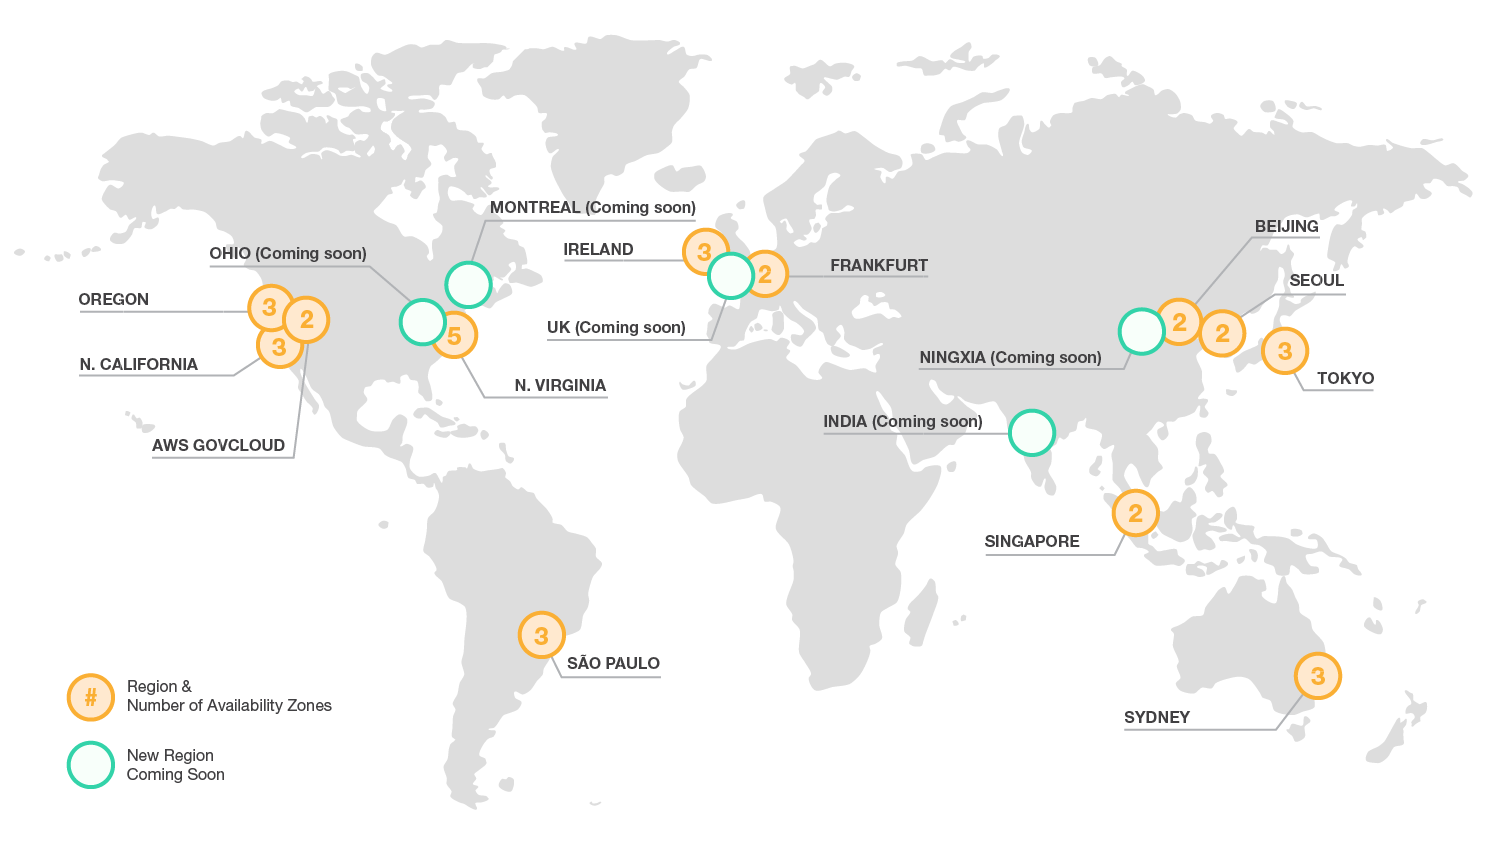
\includegraphics[width=1\textwidth]{aws-infrastructure}
	\caption{\emph{Infraestrutura Geral da Amazon Web Services \cite{awsinfra}}}
	\label{fig:awsInfra}
\end{figure}

Assim como a maioria dos serviços disponíveis para nuvem, o AWS tem diferentes valores associados aos seus recursos, incluindo uma nível de uso gratuíto, com limitações \cite{ec2price}.

Os serviços disponíveis, classificados por categoria estão representados na Figura \ref{fig:awsArq}.

\begin{figure}
	\centering
	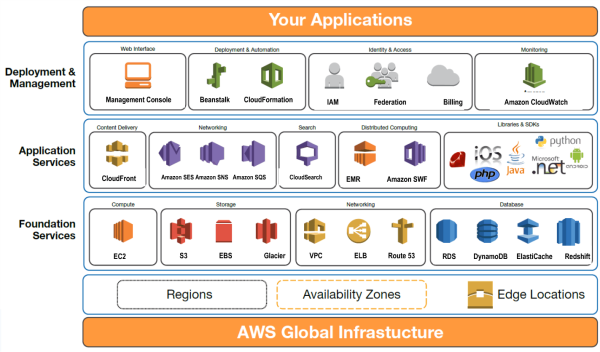
\includegraphics[width=1\textwidth]{aws-arq}
	\caption{\emph{Infraestrutura de serviços AWS \cite{awsarq}}}
	\label{fig:awsArq}
\end{figure}

\subsection{Amazon Elastic Compute Cloud - EC2}

Amazon Elastic Compute Cloud (EC2) faz parte da solução de IaaS da Amazon, provendo recursos de computação em nuvem. O serviço de EC2 conta com diversos tipos de instâncias que melhor se adequam a diferentes propósitos dentro da computação. Esses tipos são:

\begin{itemize}
\item Uso Geral
	\begin{itemize}
	\item T2 - São instâncias com menor custo. Tem capacidade de intermitência, contando com processadore Intel Xeon com até 3.3 GHz em frequência de turbo, com 1 ou 2 vCPUs com 0.5 a 8 GB de RAM. Seus principais casos de uso são ambientes de desenvolvimento, servidores de compilação, repositórios de código, sites e aplicações web de baixo tráfego, microsserviços. experimentos iniciais de produtos e pequenos bancos de dados. Utiliza Amazon EBS (Elastic Block Store) como dispositivo de armazenamento.
	\item M4 - Tem hardware mais robusto que as instãncias T2, utilizando processadores Intel Xeon® E5-2676 v3 2,4 GHz (arquitetura Haswell), com 2 a 40 vCPUs e 8 a 160 GB de RAM. Seu armazenamento em EBS é otimizado, com taxas de transferência de 450 a 4000 Mbps.
	\item M3 - Contam com processadores Intel Xeon E5-2670 v2 (Ivy Bridge) ou Xeon E5-2670 (Sandy Bridge) 2.6 GHz, com 1 a 8 vCPUs, 3.75 a 30 GB de RAM e armazenamento em SSD, seu diferencial das demais instâncias dessa categoria. Seus casos de uso mais indicados são bancos de dados de pequeno e médio porte, tarefas de processamento de dados que exigem memória adicional, grupos de armazenamento em cache e servidores de backend para SAP, Microsoft SharePoint, computação em cluster e outras aplicações empresariais.
	\end{itemize}
\item Otimizadas para computação
	\begin{itemize}
	\item C4 - Utilizam processadore Intel Xeon E5-2666 v3 (Haswell) de alta frequência otimizados especificamente para o EC2, com 2 a 36 vCPUs e 3.75 a 60 GB de RAM. O armazenamento EBS é otimizado, com taxas de transferência entre 500 e 4000 Mbps. Esta instância, assim como a C3 tem suporte aprimorado a rede, aumentando a quantidade de pacotes por segundo que podem ser enviados e recebidos.
	\item C3 - Com processadores Intel Xeon E5-2680 v2 (Ivy Bridge) de 2 a 32 vCPUs, 3,75 a 60 GB de RAM e armazenamento em SSD, seus casos de uso principais são frotas de frontend de alto desempenho, servidores da web, processamento em lotes, dados analíticos distribuídos, aplicativos científicos e de engenharia de alto desempenho, veiculação de anúncios, jogos MMO e codificação de vídeo.
	\end{itemize}
\item Otimizadas para memória
	\begin{itemize}
	\item R3 - O foco deste tipo de instância é a memória RAM, contando com valores de 15.25 a 244 GB, tem também armazenamento em SSD, tornando-a ideais para bancos de dados de alto desempenho, caches de memória distribuídos, análises em memória, montagem e análise de genomas, implementações maiores de SAP, Microsoft SharePoint e outros aplicativos empresariais.
	\end{itemize}
\item GPU
	\begin{itemize}
	\item G2 - Conta com 1 ou 4 GPUs NVidia, com 1.536 núclos CUDA e 4 GB de VRAM. Seu propósito é streaming de aplicações 3D, aprendizagem de máquina, codificação de vídeo e outras cargas de trabalho de gráficos ou computação de GPU no lado do servidor. Para isso conta com processador Intel Xeon E5-2670 (Sandy Bridge) com 8 ou 32 vCPUs, 15 ou 60 GB de RAM e armazenamento em SSD.
	\end{itemize}
\item Otimizadas para armazenamento
	\begin{itemize}
	\item I2 - Com foco em E/S, possui de 1 a 8 SSDs com 800 GB cada, processadores Intel Xeon E5-2670 v2 (Ivy Bridge) com 4 a 32 vCPUs e 30.5 a 244 GB de RAM. O suporte a rede também é aprimorado. Seus casos de uso incluem bancos de dados NoSQL, como o Cassandra e o MongoDB, bancos de dados transacionais escaláveis, armazém de dados, Hadoop e sistemas de arquivo em cluster.
	\item D2 - Instâncias de armazenamento denso, contam com processadores Intel Xeon E5-2676v3 (Haswell) com 4 a 36 vCPUs, 30.5 a 244 GB de RAM e de 3 a 20 HDDs de 2 TB. Essas instâncias são aplicáveis a armazéns de dados para processamento paralelo massivo (MPP), computação distribuída de MapReduce e Hadoop, sistemas de arquivo distribuídos, sistemas de arquivos de rede e aplicações de processamento de logs ou dados.
	\end{itemize}
\end{itemize}

Cada tipo e sub-tipo de instância tem um valor de utilização por hora diferente, crescendo consideravelmente ao se utilizar recursos melhores.

Além dos tipos de instância, estão disponíveis, na forma de AMIs \cite{ami}, diversos tipos de imagens de máquinas virtuais, baseados em diferentes sistemas operacionais. Cada uma das AMIs tem características que as tornam melhores para determinadas tarefas computacionais, geralmente diferenciadas por recursos pré-instalados e configurados.

\subsection{Amazon Virtual Private Cloud - VPC}

\begin{figure}
	\centering
	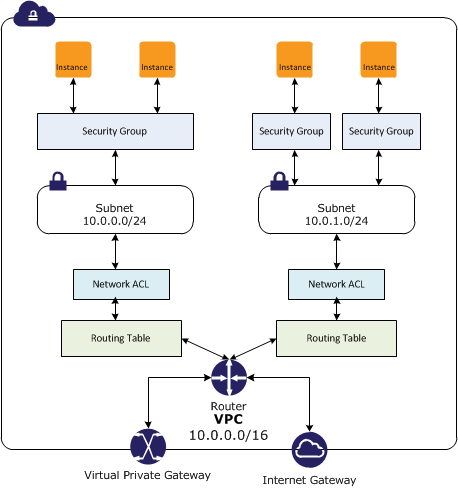
\includegraphics[width=1\textwidth]{vpc}
	\caption{\emph{Modelo de VPC com subredes, grupos de segurança, ACL, tabelas de roteamento, internet gateway e VPG \cite{vpcimg}}}
	\label{fig:vpcImg}
\end{figure}

Um recurso do AWS feito para possibilitar a divisão de outros recursos, principalmente EC2, em subnets. Com isso, é possível definir um ponto único de acesso aos demais recursos, aumentando a organização, escalabilidade e segurança da infraestrutura.

O VPC permite a personalização e divisão de endereços IP, levando a possibilidade de separação ou agrupamento de serviços. Também permite a comunicação com serviços em diferentes VPCs.

Também suporta a implantação de grupos de segurança, tabelas de roteamento e listas de controle de acesso, possibilitando a formação de uma infraestrutura robusta de rede, conforme Figura \ref{fig:vpcImg}.

\subsection{Amazon CloudFormation}

Oferece um modo simples de implantar e gerenciar um grupo de recursos do AWS, de forma previsível e replicável. O uso dessa ferramenta pode ser feita de duas formas principais, sendo elas:
\begin{itemize}
\item{Declaração estruturada em JSON}
Através de um arquivo de texto estruturado é possível descrever toda a infraesturura a ser criada, com parâmetros variáveis ou estáticos para cada recurso da pilha.

\item{CloudFormation Designer}
Uma interface gráfica que disponibiliza o drag-and-drop dos recursos afim de facilitar ainda mais a criação de uma pilha de recursos AWS. 
\end{itemize}

\subsection{Amazon Simple Storage Service - S3}

Um serviço de armazenamento da Amazon, baseado em buckets, oferece uma interface web service para armazenar e recuperar dados.

Esse serviço está bem acoplado aos demais serviços da Amazon, possibilidando o acesso via instâncias EC2, por exemplo, centralizando o armazenamento de forma confiável.

\section{Casos de Uso}

\begin{itemize}
\item System Administration, Gjovik University College por Erik Hjelmas \cite{erik} - Faz o uso de OpenStack, disponibilizando um ambiente exclusivo a cada aluno para experimentação. O ambiente provido pelo professor conta com algumas VMs de diferentes sistemas operacionais para que o aluno configure serviços como Active Directory, servidor DNS e Puppet. O uso de cloud nesse caso possibilita experimentação em um ambiente similar aos reais, apenas em menor escala.

\item Parallel Computing, Stanford University por Alex Aiken e Kunle Olukotun \cite{stanford} - Utiliza diversas infraestruturas AWS para realização de tarefas em threads, STM, MapReduce (Hadoop), OpenMP e GPGPU (CUDA).

\item Introduction to Modeling and Simulation, Massachusetts Institute of Technology por Markus J. Buehler e Jeffrey C. Grossman  \cite{starclusterMIT} - Dado o caráter naturalmente intensivo em computação da matéria, impossibilitando o uso de computadores pessoais para testes, foi implementado um cluster em cloud que acomodasse o uso por parte de todos os alunos. Porém, a manutenção de um cluster local se tornou muito expressiva, levando ao surgimento do StarCluster, uma ferramenta para criação de clusters na Amazon EC2, com AMIs personalizadas com os pacotes OpenMPI, ATLAS, NumPy/SciPy e IPython.
\end{itemize}


\section{Trabalhos Relacionados}

Existem outras ferramentas para facilitar a implantação de ambientes em EC2. Cada um desses projetos tem um foco diferente dos demais no que se refere a orquestração do ambiente, e normalmente requerem o uso de mais ferramentas auxiliares para o pleno funcionamento.

\begin{itemize}
	\item Stanford Elliot Slaughter - Baseado em um script Python para automatizar a implantação de diferentes tipos de clusters. Cada um desses tipos contém as ferramentas e ambiente preparado para um conteúdo específico dentre threads, STM, MapReduce (Hadoop), OpenMP e GPGPU (CUDA). A forma como o ambiente é implantada, e quais ferramentas instaladas, pode ser alterada por meio de modificações no script e nos arquivos de configuração.
	
	\item StarCluster \cite{starcluster} - Provê uma interface em CLI para criação, configuração, gerência e acesso a clusters na Amazon EC2. Este projeto automatiza a implantação em si, utilizando AMIs personalizadas com os pacotes OpenMPI, ATLAS, NumPy/SciPy e IPython.
\end{itemize}


\chapter{Desenvolvimento}

Este capítulo apresenta as atividades realizadas para atingir os objetivos definidos. Serão apresentados tópicos de organização da rede e integração de recursos AWS, assim como desafios de automatização encontrados.

A metodologia do projeto concentrou-se em construir a infraestrutura começando dos recursos mais gerais e andando em direção aos mais espefíficos, devido a dependências para correto funcionamento. De forma geral, o desenvolvimento seguiu esta ordem:

\begin{itemize}
	\item Virtual Private Cloud
	\item Subredes
	\item NAT
	\item Tabelas de Roteamento
	\item Instâncias
	\item Nomeação dos Hosts
	\item Configuração acesso SSH a demais hosts
	\item Instalação e Configuração de biliotecas e pacotes
	\item Acesso ao S3 
\end{itemize}


\section{Ambiente de rede}

A metodologia de desenvolvimento do projeto foi incremental, primeiramente focando em criar um ambiente base onde as intâncias serão posicionadas. Esse ambiente foi feito em volta de um VPC. Primeiramente, estabeleceu-se uma rede para endereços privados sob a qual todas as instâncias estarão alocadas. Decidiu-se pelo uso da rede 192.168.0.0/24 por ser um espaço de rede comumente utilizado para o propósito de redes privadas, além de fornecer endereços suficientes para a andamento do projeto.

Esta rede foi subdividida em duas, sendo as subredes 192.168.0.0/28 para uso das instâncias de computação e 192.168.240.0/28 para a instância com acesso externo. A instãncia colocada sob a subrede pública além de funcionar como \emph{bastion} de acesso a rede privada com as intâncias de computação, também funciona como NAT (Networking Address Translation) para citadas instâncias. Tal medida foi tomada para facilitar o controle sobre endereçamento e organização dentro do VPC.

%TODO
/* TODO: Regiões e AMIs? */

Como boa prática de segurança, foram associados grupos de segurança as subredes, tornando disponível o acesso a redes externas somente pela intância NAT, também apenas permitindo o acesso SSH via esta e demais nodos da subrede. Além dos grupos de segurança, tabelas de roteamento foram implantadas para direcionamento do tráfego de rede aos respectivos gateways. Do ponto de vista da subrede pública, esse gateway é um recurso especial da Amazon que permite o acesso a internet, chamado Internet Gateway, e do ponto de vista da subrede privada o gateway é a própria instância NAT. Uma visão geral da infraestrutura é mostrada na Figura \ref{fig:myInfra}.

\begin{figure}
	\centering
	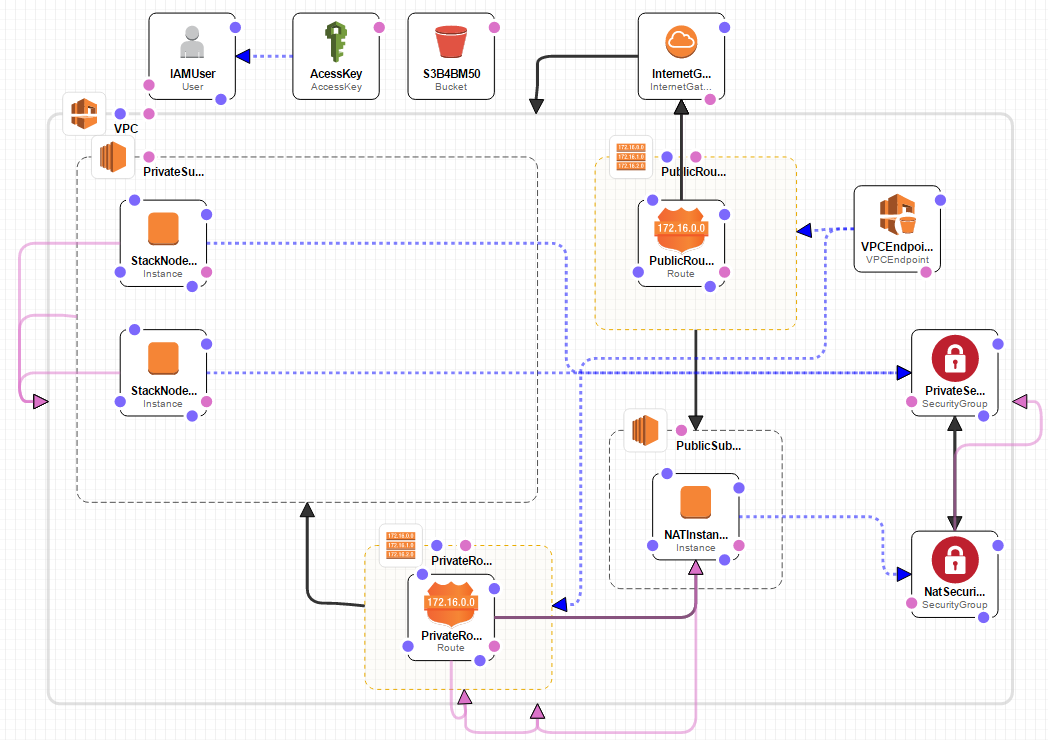
\includegraphics[width=1\textwidth]{myInfra}
	\caption{\emph{Representação da pilha de recursos}}
	\label{fig:myInfra}
\end{figure}

\section{Instâncias}

Para realização do projeto foram utilizadas instâncias do tipo \emph{t2.micro}, as quais se encaixam no plano de uso livre da AWS. Esse tipo pode ser alterado no momento da implantação do modelo, com a ressalva de que os servidores AWS da América do Sul não suportam o tipo \emph{g2}, com GPUs. Porém, essas instâncias podem ser utilizadas se a região escolhida for outra, como \emph{us-east}.

Para configuração de arquivos e instalação de pacotes necessários foram utilizados as ferramentas disponibilizadas pelo recurso Init do CloudFormation. Dentre as opções disponíveis, foram utilizadas as seguites:

\begin{itemize}
\item Packages - Provê suporte aos gerênciadores de instalação apt, msi, python, rpm, rubygems e yum. 
\item Files - Suporte para criação de arquivos e diretóríos, assim como seus conteúdos.
\item Commands - Disponibiliza a execução de comandos \emph{bash}, no caso de instâncias Linux.
\end{itemize}

Essas opção são sempre executadas pelo CloudFormation na ordem descrita, evitando a edição de pacotes ou arquivos ainda inexistentes.

\subsection{Acesso SSH}

O primeiro desafio encontrado nesta etapa foi a simplificação da configuração do acesso SSH entre as instãncias, necessário a execução de algoritmos distribuídos com MPI. Por padrão, instâncias EC2 já têm a chave pública referente ao \emph{key pair} configurado previamente a aplicação da pilha, porém, a chave privada está apenas disponível em arquivo PPK e é utilizada da máquina do usuário para acesso as instância pública. Isto não permite que as instâncias tenham acesso entre si via SSH, então foi necessário requerer a chave privada como \emph{string} no momento de implantação, salvá-las nas VMs e reorganizar a estrutura do arquivo com um script python (Figura \ref{sshKeyParser}), pois as quebras de linha são perdidas e são necessárias para a correta interpretação da chave.

Há ainda um script (Figura \ref{hostScan}) que escaneia e armazena os fingerprints de cada um dos hosts presentes na rede. Isso é feito para que não seja necessário dar permissão de acesso manualmente aos demais hosts em cada um deles, como é necessário para execuções de OpenMPI.

\begin{figure}
\centering
\begin{subfigure}[c]{1\textwidth}
\begin{lstlisting}[frame=single, language=Python, numbers=none]
import re
input = open("/home/ec2-user/.ssh/id_rsa.in").read()
bgnEnd = re.findall('-----[A-Z\s]+-----',input)
content = re.findall('-\s(.+?)\s-',input)
lines = content[0].split(" ")
outputFile = open("/home/ec2-user/.ssh/id_rsa", "w")
outputFile.write(bgnEnd[0] + '\n')
[outputFile.write(line + '\n') for line in lines]
outputFile.write(bgnEnd[1])
outputFile.close()
\end{lstlisting}
\caption{sshParser.py}
\label{sshKeyParser}
\end{subfigure}

\begin{subfigure}[c]{1\textwidth}
\begin{lstlisting}[frame=single, language=Python, numbers=none]
import re
from subprocess import check_output
input = open("/etc/hosts").read()
hosts = re.findall('\s([a-z0-9]+[0-9])\n', input)
ips = re.findall("\n(\d{1,3}\.\d{1,3}\.\d{1,3}\.\d{1,3})\s", input)
output = list()
[output.append(check_output(["ssh-keyscan", "-H", ip])) for ip in ips]
[output.append(check_output(["ssh-keyscan", "-H", host])) for host in hosts]
outputFile = open("/home/ec2-user/.ssh/known_hosts", "w")
[outputFile.write(line + '\n') for line in output]
outputFile.close()
\end{lstlisting}
\caption{sshHostScan.py}
\label{hostScan}
\end{subfigure}
\caption{Scripts de automatização}
\end{figure}

\begin{figure}
\centering
\begin{lstlisting}[frame=single, numbers=none]
"AWS::CloudFormation::Init" : {
	"config" : {
		"files" : {
			"/etc/hosts" : {
				"content" : {
					"Fn::Join" : ["\n", [
					"127.0.0.1   localhost   localhost",
					{"Fn::FindInMap":["IpAddressConfig", "Node01", "IP" ]},"  node01  node01",
					{"Fn::FindInMap":["IpAddressConfig", "Node02", "IP" ]},"  node02  node02",
					{"Fn::FindInMap":["IpAddressConfig", "Node03", "IP" ]},"  node03  node03",
					{"Fn::FindInMap":["IpAddressConfig", "Node04", "IP" ]},"  node04  node04",
					{"Fn::FindInMap":["IpAddressConfig", "Node05", "IP" ]},"  node05  node05"]]
				}
			}
		}	
	}
}
\end{lstlisting}
\caption{Edição do arquivo /etc/hosts via CloudFormation}
\label{hostFile}
\end{figure}

Outra modificação aplicada foi a edição do arquivo \verb|/etc/hosts| para adicionar \emph{alias} aos endereços das instâncias da subrede, conforme Figura \ref{hostFile}.


\subsection{Instalação de Pacotes}

%TODO outros pacotes
A imagem utilizada nas VMs já possui repositórios yum configurados, diponibilizando a instalação dos pacotes openmpi, java-devel, ant, gcc e gcc-c++.

\subsubsection{OpenMPI}

A configuração desse pacote começa com a exportação de variáveis de ambiente, indicando os \emph{wrappers} de compilação e execução. Para isso foi utilizado o recurso de execução de comandos do Init, conforme Figura \ref{openMPI}.

\begin{figure}
\centering
\begin{lstlisting}[frame=single, numbers=none]
"AWS::CloudFormation::Init" : {
	"configure" : {
		"commands" : {
			"exportOpenMPIBin" : {
				"command" : "echo \"export PATH=/usr/lib64/openmpi/bin:$PATH\" >> /home/ec2-user/.bashrc"
			},
			"exportOpenMPILib" : {
				"command" : "echo \"export LD_LIBRARY_PATH=/usr/lib64/openmpi/lib:$LD_LIBRARY_PATH\" >> /home/ec2-user/.bashrc"
			}
		}
	}
}
\end{lstlisting}
\caption{Exportação do PATH do OpenMPI}
\label{openMPI}
\end{figure}

Para sincronização dos executáveis compilados, está disponível nas máquinas virtuais a ferramenta rsync ou scp, conforme preferir o usuário.

\subsubsection{Java RMI}

Para habilitar o ambiente para a compilação de códigos em Java foi instalado o pacote java-devel, que provê o Java Development Kit (JDK). Também foi instalada a ferramenta ant, caso seja necessária.

Através do Init foi feita a exportação da variável de ambiente JAVA\_HOME para indicar o caminho do JDK ao invés do JRE préviamente indicado, conforme Figura \ref{javaHome}.

\begin{figure}
\centering
\begin{lstlisting}[frame=single, numbers=none]
"exportJavaHome" : {
	"command" : "echo \"export JAVA_HOME=/usr/lib/jvm/java-openjdk/\" >> /home/ec2-user/.bashrc"
}
\end{lstlisting}
\caption{Exportação do PATH do JDK}
\label{javaHome}
\end{figure}


\subsection{Upload de Arquivos}

Com o intuito de integrar essa parte do processo de desenvolvimento, foi criado um VPC Endpoint (Figura \ref{vpcEndpoint} que cria um ponto de acesso ao S3. Para usufruir dos serviços, porém, foi necessária a criação de um usuário IAM e chaves de acesso ao serviço (Figura \ref{accessKey}, assim como a configuração (Figura \ref{awsCredentials} destas nas instâncias.

\begin{figure}
\centering

\begin{subfigure}[c]{1\textwidth}
\begin{lstlisting}[frame=single, numbers=none]
"VPCEndpointS3" : {
	"Type" : "AWS::EC2::VPCEndpoint",
	"Properties" : {
		"ServiceName"		: "com.amazonaws.sa-east-1.s3",
		"VpcId"				: { "Ref": "VPC" },
		"RouteTableIds"	: [ { "Ref": "PrivateRouteTable"  }, { "Ref": "PublicRouteTable"  } ]
	}
}
\end{lstlisting}
\caption{VPC Endpoint}
\label{vpcEndpoint}
\end{subfigure}

\begin{subfigure}[c]{1\textwidth}
\begin{lstlisting}[frame=single, numbers=none]
"IAMUser" : {
	"Type" : "AWS::IAM::User",
	"Properties" : {
		"Path" : "/"
	}
},		
"AcessKey" : {
	"Type" : "AWS::IAM::AccessKey",
	"Properties" : {
		"UserName" : { "Ref" : "IAMUser" }
	}
} 
\end{lstlisting}
\caption{Usuário IAM e Chave de Acesso}
\label{accessKey}
\end{subfigure}

\begin{subfigure}[c]{1\textwidth}
\begin{lstlisting}[frame=single, numbers=none]
"/home/ec2-user/.aws/credentials" : {
	"content" : {
		"Fn::Join" : ["", [
			"[default]\n",
			"aws_access_key_id=", { "Ref" : "AcessKey" }, "\n",
			"aws_secret_access_key=", { "Fn::GetAtt" : [ "AcessKey", "SecretAccessKey" ] }					
		]]
	}
}
\end{lstlisting}
\caption{AWS Credentials}
\label{awsCredentials}
\end{subfigure}
\caption{Configuração de acesso ao S3}
\end{figure}

O acesso pode ser feito via API da Amazon, pré instalada na AMI, ou via GET/wget.

A automatização da criação do bucket em si enfrenta o porém de que estes devem ter nomes diferentes dentre todos os buckets do S3.


\chapter{Resultados}

Até o momento este projeto possibilita a criação de uma pilha de recursos estática, pronta para desenvolvimento paralelo e distribuído com OpenMP, MPI e RMI.

O acesso a essa pilha de recursos se dá por SSH, primeiramente acessando a instância bastion, que tem endereço IP público e a partir dela, também por SSH, pode-se acessar as demais instâncias destinadas ao desenvolvimento, utilizando o prefixo \emph{node} acompanhado por número idendificador de dois dígitos, por exemplo \emph{ssh node01}.

Uma vez acessada uma instância de computação, pode-se acessar as demais da mesma forma descrita acima. O ambiente também já está pronto para compilação e execução de códigos MPI, RMI e OpenMP, sem interface gráfica. A tranferência de dados da máquina do usuário para a instãncia pode ser feita através do upload de arquivos para um bucket da Amazon S3, o qual precisa ser criado por cada usuário, e então fazendo o download na instãncia utilizando \emph{wget} ou comandos do Amazon CLI.

Os comandos importantes para acesso ao S3 são \emph{aws s3 cp s3://nome-do-bucket/arquivo-remoto arquivo-local}, para download de um arquivo único, ou \emph{aws s3 sync s3://nome-do-bucket pasta-local} para sincronizar todo o bucket para um diretório local. O processo de upload de arquivos da instância para o S3 pode ser feito invertendo a posição dos caminhos locais e remotos em ambos os comandos. Todas as configurações e permissões de acesso para realizar esse processo são automaticamente realizadas ao se lançar a pilha de recursos.

\chapter{Conclusão}

Esse projeto tinha como propósito criar um ambiente facilmente implantável, escalável e replicável, que simule ambiente reais de desenvolvimento, para uso no processo de ensino de conteúdos de computação paralela e distribuída.

A etapa de desenvolvimento se deu através do planejamento da infraestrutura de rede de forma escalável e simples. Assim como pelo levantamento de quais são as ferramentas necessárias dentro do ambiente para execução dos códigos alvo para então realizar a instalação automatizada das bibliotecas e aplicativos.

Ao fim desta etapa, foi atingido o objetivo de criação de um ambiente replicável e facilmente implatável, porém a escalabilidade ainda depende de modificações diretamente em código.

Como continuidade, será elaborada uma interface para modificação e expansão do modelo estático produzido até o momento, para melhor atender demandas individuais.


\setlength{\baselineskip}{\baselineskip}
\bibliographystyle{abnt}
\bibliography{references}

\end{document}
